\documentclass[
	12pt,
	a4paper,
	bibtotoc,
	cleardoubleempty, 
	idxtotoc,
	openright
	final,
	listof=nochaptergap,
	]{scrbook}
\usepackage{cmap}
\usepackage[T1]{fontenc}
\usepackage[utf8]{inputenc}
\usepackage{natbib}

% ##################################################
% Unterstuetzung fuer die englishe Sprache
% ##################################################
\usepackage[english]{babel}
\usepackage{graphicx}
\usepackage{wrapfig}

% ##################################################
% Dokumentvariablen
% ##################################################

% Persoenliche Daten
\newcommand{\docNachname}{Gilli}
\newcommand{\docVorname}{Stephan}
\newcommand{\docStrasse}{Lerchenauerstraße 218}
\newcommand{\docOrt}{München}
\newcommand{\docPlz}{80395}
\newcommand{\docEmail}{stephan.gilli@hs-furtwangen.de}
\newcommand{\docMatrikelnummer}{000000}

% Dokumentdaten
\newcommand{\docTitle}{The digital twin as a central control element in supply-oriented value networks}
\newcommand{\docUntertitle}{using the Asset Administration Shell} % Kein Untertitel
\newcommand{\docUntertitle}{UNTERTITEL}
\newcommand{\docArtDerArbeit}{Masterthesis}
% Software-Produktmanagement Bachelor, Advanced Computer Scinece Master
\newcommand{\docStudiengang}{Sales \& Service Engineering}
\newcommand{\docAbgabedatum}{xx.xx.2022}
\newcommand{\docErsterReferent}{Prof. Dr. Harald Kopp}
%\newcommand{\docZweiterReferent}{-} % Wenn es nur einen Betreuer gibt
\newcommand{\docZweiterReferent}{}

% ##################################################
% Allgemeine Pakete
% ##################################################

% Abbildungen einbinden
\usepackage{graphicx}

% Zusaetsliche Sonderzeichen
\usepackage{dingbat}

% Symbole Haken und X [OPTIONAL]
%\usepackage{pifont}
%\newcommand{\cmark}{\ding{51}}
%\newcommand{\xmark}{\ding{55}}

% Farben
\usepackage{color}
\usepackage[usenames,dvipsnames,svgnames,table]{xcolor}

% Maskierung von URLs und Dateipfaden
\usepackage[hyphens]{url}

% Deutsche Anfuehrungszeichen
\usepackage[babel, german=quotes]{csquotes}

% Pakte zur Index-Erstellung (Schlagwortverzeichnis)
\usepackage{index}
\makeindex


% ##################################################
% Seitenformatierung
% ##################################################
\usepackage[
	portrait,
	inner=2.5cm,
	outer=2.5cm,
	top=3cm,
	bottom=2cm,
	%showframe, %Aktivieren um Seitengrenzen anzuzeigen
	%includeheadfoot
	]{geometry}

% ##################################################
% Kopf- und Fusszeile
% ##################################################

\usepackage{fancyhdr}

\pagestyle{fancy}
\fancyhf{}
\fancyhead[EL,OR]{\sffamily\thepage}
\fancyhead[ER,OL]{\sffamily\nouppercase{\leftmark}}

\fancypagestyle{headings}{}

\fancypagestyle{plain}{}

\fancypagestyle{empty}{
  \fancyhf{}
  \renewcommand{\headrulewidth}{0pt}
}

%Speichert \chaptermark in \oldchaptermark damit 
% es für die Anhänge zurückgesetzt werden kann
\let\oldchaptermark\chaptermark

%Kein "Kapitel # NAME" in der Kopfzeile
\renewcommand{\chaptermark}[1]{
	\markboth{#1}{}
   	\markboth{\thechapter.\ #1}{}
}

% ##################################################
% Schriften
% ##################################################

% Stdandardschrift festlegen
\renewcommand{\familydefault}{\sfdefault}

% Standard Zeilenabstand: 1,5 zeilig
\usepackage{setspace}
\onehalfspacing 

% Schriftgroessen festlegen
\addtokomafont{chapter}{\sffamily\large\bfseries} 
\addtokomafont{section}{\sffamily\normalsize\bfseries} 
\addtokomafont{subsection}{\sffamily\normalsize\mdseries} 
\addtokomafont{caption}{\sffamily\normalsize\mdseries} 

%Einrücken von Absätzen deaktivieren
\setlength{\parindent}{0pt}

%Zeilenabstand bei abstätzen
\usepackage{parskip}

% ##################################################
% Inhaltsverzeichnis / Allgemeine Verzeichniseinstellungen
% ##################################################

\usepackage{tocloft}

% Punkte auch bei Kapiteln
\renewcommand{\cftchapdotsep}{3}
\renewcommand{\cftdotsep}{3}

% Schriftart und -groesse im Inhaltsverzeichnis anpassen
\renewcommand{\cftchapfont}{\sffamily\normalsize}
\renewcommand{\cftsecfont}{\sffamily\normalsize}
\renewcommand{\cftsubsecfont}{\sffamily\normalsize}
\renewcommand{\cftchappagefont}{\sffamily\normalsize}
\renewcommand{\cftsecpagefont}{\sffamily\normalsize}
\renewcommand{\cftsubsecpagefont}{\sffamily\normalsize}

%Zeilenabstand in den Verzeichnissen einstellen
\setlength{\cftparskip}{.5\baselineskip}
\setlength{\cftbeforechapskip}{.1\baselineskip}

%Einrücken von Absätzen deaktivieren
%\setlength{\parindent}{0pt}

%Zeilenabstand bei abstätzen
\usepackage{parskip}

% ##################################################
% Abbildungsverzeichnis und Abbildungen
% ##################################################

\usepackage{caption}

\usepackage{wrapfig}

% Nummerierung von Abbildungen
\renewcommand{\thefigure}{\arabic{figure}}
\usepackage{chngcntr}
\counterwithout{figure}{chapter}

% Abbildungsverzeichnis anpassen
\renewcommand{\cftfigpresnum}{Abbildung }
\renewcommand{\cftfigaftersnum}{:}

% Breite des Nummerierungsbereiches [Abbildung 1:]
\newlength{\figureLength}
\settowidth{\figureLength}{\bfseries\cftfigpresnum\cftfigaftersnum}
\addtolength{\figureLength}{2mm} %extra offset
\setlength{\cftfignumwidth}{\figureLength}
\setlength{\cftfigindent}{0cm}

% Schriftart anpassen
\renewcommand\cftfigfont{\sffamily}
\renewcommand\cftfigpagefont{\sffamily}

%standardpfad anpassen
\graphicspath{ {../src/content/pictures/} }

% ##################################################
% Tabellenverzeichnis und Tabellen
% ##################################################

% Nummerierung von Tabellen
\renewcommand{\thetable}{\arabic{table}}
\counterwithout{table}{chapter}

% Tabellenverzeichnis anpassen
\renewcommand{\cfttabpresnum}{Tabelle }
\renewcommand{\cfttabaftersnum}{:}

% Breite des Nummerierungsbereiches [Abbildung 1:]
\newlength{\tableLength}
\settowidth{\tableLength}{\bfseries\cfttabpresnum\cfttabaftersnum}
\addtolength{\tableLength}{3mm} %extra offset
\setlength{\cfttabnumwidth}{\tableLength}
\setlength{\cfttabindent}{0cm}

%Schriftart anpassen
\renewcommand\cfttabfont{\sffamily}
\renewcommand\cfttabpagefont{\sffamily}

% Unterdrueckung von vertikalen Linien
\usepackage{booktabs}

%Multi row für spezifische zellen
\usepackage{multirow}

%Additional table package
\usepackage{tabu}

% ##################################################
% Appendix
% ##################################################

%Calc packet für berechnungen
\usepackage{calc}

%Appendix paket, setzen der flags für das TOC
\usepackage[toc,title,titletoc]{appendix} 

%Umbenennen der überschrift für die Anhänge 
\renewcommand{\appendixtocname}{Anhänge}

%Befehl für einen neuen Bericht und die erste seite als bild
\newcommand{\appendixsection}[2]{
\section{#1}
\appendixsingle{#2}
}

%Befehl für einzelne seite als bild eingefasst, damit überschrift und kopfzeile
% bestehen bleibt. 
\newcommand{\appendixsingle}[1]{
\vspace{-10cm}
\vfill
\mbox{}\hspace{-1.5cm}\includegraphics[width=\linewidth+3cm]{#1}\hspace{-1.5cm}\mbox{}
\vspace{-10cm}
\vfill
\mbox{}
}

%Datenträger Tabelle
\definecolor{lightgray}{gray}{0.85}
\definecolor{ultralightgray}{gray}{0.95}
\definecolor{mygray}{gray}{0.70}

% ##################################################
% Theoreme
% ##################################################
  	
% Umgebung fuer Beispiele
\newtheorem{beispiel}{Beispiel}

% Umgebung fuer These
\newtheorem{these}{These}

% Umgebung fuer Definitionen
\newtheorem{definition}{Definition}
  	
% ##################################################
% Literaturverzeichnis
% ##################################################

\usepackage{bibgerm}

% ##################################################
% Abkuerzungsverzeichnis
% ##################################################

\usepackage[printonlyused]{acronym}

% ##################################################
% PDF / Dokumenteninternelinks
% ##################################################

\usepackage[
	colorlinks=false,
   	linkcolor=black,
   	citecolor=black,
  	filecolor=black,
	urlcolor=black,
    bookmarks=true,
    bookmarksopen=true,
    bookmarksopenlevel=3,
    bookmarksnumbered,
    plainpages=false,
    pdfpagelabels=true,
    hyperfootnotes,
    pdftitle ={\docTitle},
    pdfauthor={\docVorname~\docNachname},
    pdfcreator={\docVorname~\docNachname}]{hyperref}

% ####################################################
% Command für einfache Quellenangabe bei Bilder, etc.
% ####################################################

\newcommand{\source}[1]{\caption*{Source: {#1}} }

% ###################################################
% Util Packages
% ###################################################
\usepackage{subfigure}



\begin{document}

\setcounter{secnumdepth}{3}


% Titelblatt
\begin{titlepage}
\pagestyle{empty}

% ##################################################
% HFU-Logo einbinden
% ##################################################
\begin{flushright}
\begin{figure}[ht]
\flushright

\includegraphics[height=3cm]{content/pictures/hfu.jpg}
\end{figure}
\end{flushright}

% ##################################################
% Titel
% ##################################################
\begin{center}
{\fontsize{18}{22} \selectfont \docArtDerArbeit}\\[5mm]
{\fontsize{18}{22} \selectfont im Studiengang} \\[5mm]
{\fontsize{18}{22} \selectfont \docStudiengang}\\
\vspace{1cm}
\begin{onehalfspace}
{\fontsize{22}{26} \selectfont \textbf{\docTitle}}\\[5mm]
{\fontsize{18}{22} \selectfont \docUntertitle}


\end{onehalfspace}
\end{center}

% ##################################################
% Zusatzinformationen
% ##################################################
\vfill
\begin{center}
\begin{tabular}{lcl}
Dozent  		&:& \docErsterReferent 	\\ \\
Koreferent 		&:& \docZweiterReferent \\ \\	
Vorgelegt am 	&:& \docAbgabedatum 	\\ \\
Vorgelegt von 	&:& \docVorname~\docNachname\\
				& & Matrikelnummer: \docMatrikelnummer\\
				& & \docStrasse,~\docPlz~\docOrt	\\
				& & \docEmail			
\end{tabular}
\end{center}
\end{titlepage}

\frontmatter
\pagenumbering{Roman}

% Abstract
\chapter*{Abstract\markboth{Abstract}{}}
\addcontentsline{toc}{chapter}{Abstract}


\let\cleardoublepage\clearpage

\phantomsection
\addcontentsline{toc}{chapter}{Table of Contents}
\tableofcontents
\let\cleardoublepage\clearpage

\newpage
\phantomsection 
\addcontentsline{toc}{chapter}{\listfigurename} 
\listoffigures
\let\cleardoublepage\clearpage

\newpage
\phantomsection
\addcontentsline{toc}{chapter}{\listtablename}
\listoftables
\let\cleardoublepage\clearpage

\newpage
% Abkürzungsverzeichnis
\chapter*{List of Abbreviations\markboth{List of Abbreviations}{}}
\addcontentsline{toc}{chapter}{List of Abbreviations}

\begin{acronym}
\acro{AAS}{Asset Administration Shell}
\acro{API}{Application Programming Interface}
\acro{BOM}{Bill of Material}
\acro{BPM}{Business Process Management}
\acro{BPMS}{Business Process Management Systems}
\acro{CPS}{Cyber Physical System}
\acro{DT}{Digital Twin}
\acro{ERP}{Enterprise Resource Planning}
\acro{HFU}{Hochschule Furtwangen University}
\acro{I4.0}{Industry 4.0}
\acro{IIOT}{Industrial Internet of Things}
\acro{ISA}{International Society of Automation}
\acro{MQTT}{Message Queuing Telemetry Transport}
\acro{OPCUA}{OPC Unified Architecture } 
\acro{PLC}{Programmable Logical Controller}
\acro{RAMI4.0}{Reference Architecture Model Industrie 4.0}
\acro{SOA}{Service Oriented Architecture}
\acro{SBC}{Single Board Computer}
\acro{VDMA}{Verband Deutscher Maschinen- und Anlagenbau}
\acro{ZVEI}{Zentralverband der Elektroindustrie}
\end{acronym}
\let\cleardoublepage\clearpage

\mainmatter

% Main Content goes here 
\chapter{Introduction} \label{chap:introduction}
This chapter first gives an overview of the motivation and background of the thesis. Subsequently, the research questions are derived and expected results are considered in more detail. Finally, a summary of the structure and chapters is given.

\section{Motivation}
In recent years, the interest in \ac{I4.0} has increased rapidly, both in science as well as in industry. \ac{I4.0} describes the vision of a global network in which machines, robots, warehousing systems and humans can autonomously interact with each other in order to control physical resources and processes. This is made possible in particular by the \ac{IIOT}, in which a large number of devices such as RFID-readers, wireless sensors or cameras collect data on specific environmental conditions of assets. The autonomous interaction of participants and components in the value chain transforms production facilities into smart factories \cite[p. 20]{Acatech2013Recommendations4.0}. Smart factories enable end-to-end engineering by connecting the digital and physical world both, horizontally and vertically along the value chain, but in particular across company boundaries \cite[p. 859]{Uslander2015ReferenceApproach}. This gives rise to new forms of collaboration such as value networks. The components and systems of smart factories should be able to make autonomous decisions based on provided information, execute functions regarding their capabilities, as well as autonomously influence production, order or logistic processes. For this reason, autonomously acting components and systems based on \ac{IIOT} technology are seen as the key enabler for \ac{I4.0}. They will have far-reaching effects on business and production processes. One term that is often mentioned in this context is that of a \ac{CPS}. A \ac{CPS} describes the networking of the physical world of machines, plants and devices with the virtual world \cite{Lee2008CyberBerkeley}. The terms smart factory and \ac{CPS} are therefore used interchangeably in this thesis.

Smart factories will open up new use cases for companies of various industries and sectors. In particular the following should be mentioned:
\begin{itemize}
    \item[] \textbf{Plug and produce} Plug and produce describes the ability of a production resource to configure itself, based on its environment conditions and integrate itself correctly into the running production process without manual efforts and changes \cite[p. 146]{Ye20204.0}. This increases the flexibility of manufacturing processes. Digitally connected, the process steps of a production line can be better coordinated, which results in better utilization of available machine capacities, shorter setup-times and less manual intervention. \cite[p. 16]{Acatech2013Recommendations4.0}. 
    \item[] \textbf{Lot Size One} Lot Size One production describes the ability of a production line, to produce each product or item according to the individual buyer's specification. The modularization allows the production of individual products in small quantities at affordable prices by using automated engineering and production capabilities \cite[p. 15]{Acatech2013Recommendations4.0}.
    \item[] \textbf{Service Oriented Business Models} Service oriented business models describe the ability of a company to sell the products usage or performance rather than the product itself, which generates new sources of competitiveness. By using runtime or engineering data to improve maintenance or predict machine fail over, new services can be offered \cite{Bendig2021Equipment-as-a-ServiceIndustry}.
\end{itemize}

However, to realize the horizontal and vertical integration of all components and systems an operational end-to-end communication, also known as interoperability, must be achieved \cite[p. 858]{Uslander2015ReferenceApproach}. This assumes a common language, with consistent vocabulary, semantics and rules, so that independent systems, components as well as humans can communicate with each other. In order to enable a uniform language for the interaction of different stakeholders, numerous standardization efforts by different professional associations such as \ac{ZVEI} and \ac{VDMA} have been undertaken. To focus standardization efforts and ensure a coordinated development, the Plattform Industry 4.0 was founded in 2013. In a first step, a reference architecture model was published in 2016. \ac{RAMI4.0} lays the foundation for a cross-industry discussion about the complex tasks and contexts regarding the implementation of \ac{I4.0} \cite[p. 4]{Heidel2017ReferenzarchitekturmodellIndustrie4.0Komponente}. One of the key concepts of \ac{RAMI4.0} is the \ac{I4.0} component with the \ac{AAS}. The \ac{AAS} is the implementation of the \ac{DT} in the context of \ac{I4.0}. The \ac{AAS} enables a vendor and technology independent virtual representation of physical assets according to defined semantic standards and rules \cite[p. 5]{Wagner2017ThePlant}. The \ac{AAS} acts as an interface between different components and processes and stores all necessary properties and data about a physical asset over its life cycle. The \ac{AAS} makes it possible to integrate value-added services into distributed \ac{CPS} so that new business models can emerge within and across companies. With its cooperation possibilities, the \ac{AAS} will therefore become the basis for all new use cases realized in the fourth industrial revolution \cite[p. 67]{Heidel2017ReferenzarchitekturmodellIndustrie4.0Komponente}.    

Given the fact, that one of the visions of \ac{I4.0} is to make production more flexible and autonomous by enabling decentralized execution of processes, current concepts in the field of engineering and production fall short. To understand this in more detail, a closer look needs to be taken at the current state of the automation pyramid, defined by the \ac{ISA} \cite{InternationalSocietyofAutomation2008EnterpriseIntegration}. Currently, given the production line equipped with some robotic and manual workstations, an engineer needs to obtain requirements from the office floor, in order to design the entire production process and assign the required production resources. The requirements can come hereby in any form, without generally applicable semantic standards, and can be expressed in some supportive high-level languages like GANT- or flowcharts or lists of physical equipment (Bill of Material). The required manufacturing process is then implemented using dedicated \ac{PLC} which execute the corresponding process steps. The results of the individual process steps are reported then to a central higher level supervision and control system for monitoring \cite[p.2, 3]{Wagner2017ThePlant}. The intelligence and know-how to setup and run a production process lies exclusively with the engineer. Each change to the production line and its possible side-effects must be planned in advance. Consequently the production line is highly tailored to a specific product and manufacturing resource and is only flexible to the extent that it was planned in advance \cite[p. 1]{Keddis2015Capability-basedSystems}. In order to realize the advantages of \ac{I4.0}, the allocation of production resources and the definition of the production process can no longer be done manually. This must be realized automatically during operational use \cite[p. 9]{Bock2016Weiterentwicklung4.0-Komponenten}.

To address the shortcomings, companies are moving towards implementing a \ac{SOA}. In a \ac{SOA}, the centralized control of business and manufacturing processes is replaced by a distributed architecture \cite[p. 861]{Uslander2015ReferenceApproach}. This approach is also called capability based engineering and operation of systems \cite[p. 5]{Bayha2020DescribingComponents}. For this purpose, the individual control components and information systems offer their functionalities and capabilities in the form of web services, which communicate with each other via a uniform interface. This is realized by the \ac{DT}, respectively the \ac{AAS} in \ac{I4.0}. A key characteristic of this approach, compared to the current state is, that the services in a \ac{SOA} are loosely coupled. This means, that all services can perform their capabilities independently of each other without being aware of the current production process and product to produce. This leads to a high degree of modularity and resuability and removes possible side-effects when changing the business or manufacturing process \cite[p. 491]{Schicke2020EnablingTwins}. Distributed architectures and especially the \ac{AAS} are thus moving into focus and increasingly take over tasks that were previously performed by centrally located systems. To realize this, capabilities and processes need to be associated with the \ac{AAS} so that they can be executed at the right time in the right way. This way, several temporarily interconnected components can perform more complex operations together as part of a machine or plant network. However, according to the current state of research, \ac{RAMI4.0} and the \ac{AAS} offer only limited methods for designing, operating and monitoring the composition of loosely coupled services in order to execute business and production processes. 

A widely used method for designing, operating and controlling processes within a company is \ac{BPM}. \ac{BPM} enables companies to ensure consistent outcomes and take advantage of improvement opportunities regarding their business processes \cite[p. 1]{Dumas2018FundamentalManagement}. The improvements can be of a very different nature, such as cost reduction, efficiency gains or improved quality due to minimization of error rates. To execute the processes at the right time by the right resource, \ac{BPMS} are used. In addition to their executive function, \ac{BPMS} also document the execution of processes which forms the basis for subsequent analyses and improvements of the processes \cite[p. 345]{Dumas2018FundamentalManagement}. The literature already contains approaches on how BPM can be applied in \ac{I4.0} scenarios. \citet[p. 1444]{Schonig2020IoTExecution} show that by integrating machine and sensor data in a process model, a more comprehensive view on a business and manufacturing processes can be achieved as well as cost reductions and efficiency gains can be realized. For example, when producing raw material on multiple machines, quality problems can be identified more quickly due to the available real-time data and the process can be adjusted  automatically without losing time. Thereby the authors point out, that one of the central requirement during the integration of sensor and machine data into a \ac{BPM} model is the provision of context-specific knowledge describing the machine and sensor data \cite[p. 1447]{Schonig2020IoTExecution}. \citet[p. 2]{Jaenisch2017TheChallenges} point out benefits by using \ac{BPM} to orchestrate processes in a \ac{CPS}, in regards to the the planning, execution and monitoring of distributed production processes. For example, sensor and machine data can be used to detect discrepancies between a predefined process model and the actual process. Also the planning of production processes in distributed systems can be improved, as the individual services in the production process know the goals and procedures in terms of time and cost of other services in the system and can act accordingly. However, they also point out that \ac{BPM} and \ac{CPS} can only mutually benefit from each other if the raw sensor and machine data are enriched with a semantic model so that they become interpretable.    

The increasing decentralization and the move towards a \ac{SOA} shows that there is a particular need in the context of how future business and production processes are planned, executed and optimized in a \ac{I4.0} system. This applies in particular to the orchestration of the components and services in a distributed \ac{CPS}. According to the literature \ac{BPM} could play a role in the planning, execution and orchestration of the services. This assumption requires, that the services are reachable by a standardized interface and thus the sensor and machine data are interpretable by means of a semantic model. \ac{RAMI4.0} and the \ac{AAS} enable the semantic description of sensor and machine data by offering a standardized interface. The \ac{AAS} component could thus become the central control element between the business and manufacturing processes to be executed and the services that expose the functionalities and capabilities of an asset. However, currently the concepts of the \ac{AAS} and \ac{BPM} are defined at different abstraction levels and there is so far no explicit link to bridge the gap. Further research is needed to determine whether BPM can be used to plan, execute and orchestrate services in a decentralized \ac{CPS} with the \ac{AAS} as the central connection and control element between the process steps and the resources required for them. 

\section{Research Question} \label{sec:research-question}
This thesis tries to work out an approach how the planing, execution and orchestration of decentralized services with the help of \ac{BPM} and \ac{AAS} in value networks can be implemented based on the \ac{RAMI4.0} architecture.

To this end, the following questions are to be answered in the course of this thesis:

\begin{itemize}
    \item [] \textbf{Question 1:} \textit{How can \ac{BPM} be classified in the six layers of \ac{RAMI4.0}?}
    
    The first question is intended to provide information about which general requirements \ac{RAMI4.0} defines for the six layers of the architecture axis and to what extend \ac{BPM} can be found in them. To this end, the available information in the individual layers and the dependencies between them will be examined in more detail. The main focus will be on determining the relevant information flow between the layers. The result will clarify the functional requirements defined by \ac{RAMI4.0} and how they can be taken into account in \ac{BPM}.
    
    \item [] \textbf{Question 2:} \textit{How can a link between a process and the required services involved in it be established with the help of the \ac{AAS}?}
    
    The second question builds on the results of the first question and takes an even closer look at the \ac{I4.0} component and the \ac{AAS} contained therein. For this purpose, the structure, contents and characteristic features of the \ac{AAS} are elaborated. Furthermore, a closer look at the interaction model between two \ac{AAS} is taken. In order to determine the link between process and service, the \ac{I4.0} component is mapped in the six layers of \ac{RAMI4.0}. The result of the question will shed light on when and how a service can be an active process participant.
    
    \item[] \textbf{Question 3:} \textit{How can a concrete integration of \ac{BPM} in the \ac{AAS} be realized based on the six layers of \ac{RAMI4.0}?}
    
    The third question summarizes the findings from the previous questions and attempts to make a proposal for the integration of \ac{BPM} into the \ac{AAS} . For this purpose, the functional requirements defined in question 1 and the features and characteristics of the \ac{AAS} identified in question 2 are transferred into a concrete application model. The application model is based on the six layers of \ac{RAMI4.0}. 

\end{itemize}

\section{Structure}
The approach and further chapters of the thesis are as follows:
\begin{itemize}
    \item[] In chapter two, a literature review is carried out, to explain the basic concepts of \ac{I4.0} in greater detail. First, value networks with reference to \ac{I4.0} are explained and the resulting need for a reference architecture model is derived, which is presented afterwards. This is followed by an introduction to the general concepts of a \ac{DT} and the implementation of the \ac{DT} in the \ac{I4.0} component.
    
    \item[] The third chapter takes a closer look at the \ac{AAS}. For this reason, the functional requirements of an \ac{AAS} in \ac{RAMI4.0} are examined and elaborated in greater detail. In particular, the different forms of the \ac{AAS} in value networks will be examined on the basis of defined use cases. Finally, the \ac{AAS} will be mapped into the six layers of \ac{RAMI4.0}.
    
    \item[] In the fourth chapter, the application model based on the obtained results from the previous chapters is presented. For this purpose, a technology-neutral architecture is proposed for implementation, which is backed up with a 4-step implementation guide. The fifth chapter summarizes the results obtained and provides an outlook on further topics. 
\end{itemize}


\section{Definition of terms}
In order to have a consistent definition of important terms within this thesis, some are defined once here:
\begin{itemize}
    \item[] \textbf{Component} The term component is used to describe devices such as a sensor, actuator as well as machines, industrial controllers or software processes and agents. A smart component is characterized by the fact that it provides relevant information, such as production parameters or services, such as the independent determination of the operating status via a communication interface in a standardized form with other system participants.
    \item[] \textbf{Asset} The term asset is used to describe an object in the physical world that has a certain business value for a company and can be described on the basis of properties and characteristics.
\end{itemize}
\chapter{Basics}
\let\cleardoublepage\clearpage
\chapter{Asset Administration Shell} \label{chap:aas-and-rami}
The previous chapter \ref{chap:basics} described the vertical axis of \ac{RAMI4.0}, which provides insights about the information stored about an asset in \ac{RAMI4.0}. The exchange of information between the layers either takes place within the layer or between neighboring layers. As mean for exchanging information between the layers the \ac{I4.0} component with its \ac{AAS} was introduced. This chapter goes into detail about the \ac{AAS}, works out the characteristic features and classifies the \ac{AAS} in \ac{RAMI4.0}.


\section{General Aspects} \label{sec:assetadministrationshell}
As outlined in chapter \ref{sec:digitaltwin}, the \ac{AAS} is the realization of the \ac{DT} in the context of \ac{I4.0} and contains all relevant data and functions necessary to represent the physical asset in the information world. Figure \ref{fig:structureaas} shows the \ac{AAS} with its structure and characteristic features.

\begin{figure}[h]
\centering
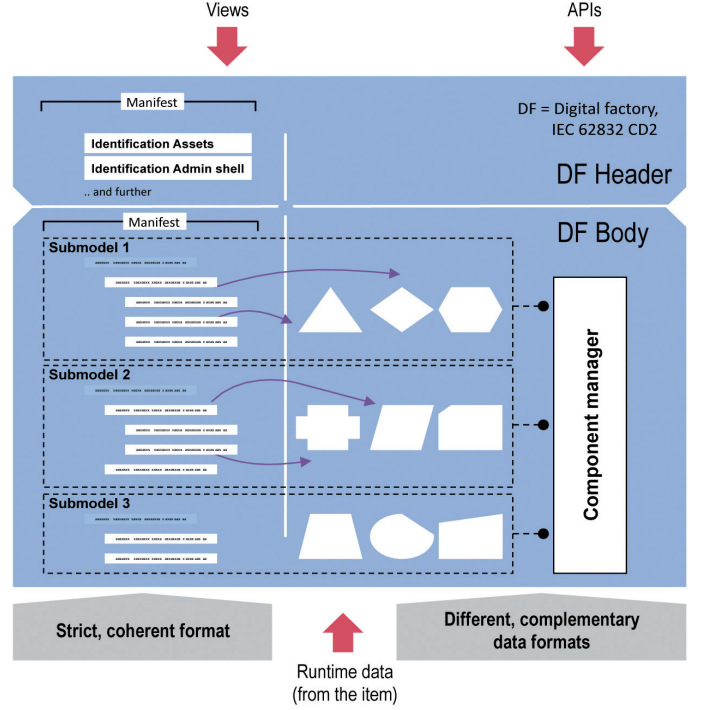
\includegraphics[scale=0.8]{content/pictures/structure_aas_zvei.png}
\caption{Structure of the Asset Administration Shell}
\source{\cite[p. 5]{Koschnick2016Beispiele4.0-Komponente-Basisteil}}
\label{fig:structureaas}
\end{figure}

The \ac{AAS} consists of two parts: The manifest and the component manager. The manifest contains metadata regarding the \ac{I4.0} component, such as a global unique identifier that can be used to identify the \ac{I4.0} component in the value chain. In addition, the metadata provides information whether the \ac{I4.0} component is of type or instance according to the life cycle \& value stream axis in \ac{RAMI4.0}. The component manager provides the uniform interface of the \ac{AAS}, through which the essential properties and functions of the asset can be realized. The goal of the \ac{AAS} is to accommodate as many application scenarios and use cases as possible, so that a variety of different data and functions can be provided \cite[p. 25]{Adolphs2016StructureComponent}. Complex machines, plants and components often consist of several thousand properties in different variants and offer a multitude of functionalities. To group the properties and functions according to their use case, they are represented in submodels within the \ac{AAS}. A submodel describes exactly one property or function of the \ac{I4.0} component in a semantically uniform way. A submodel can model general aspects of the asset or specialized capabilities such as drilling, milling or analytical aspects used for predictive maintenance \cite[p. 23]{Belyaev2021ModellingECLASS}. By encapsulating the properties and functions in independent submodels, the integration of the \ac{I4.0} component in \ac{SOA} is made possible. This way, other \ac{I4.0} components can use the component manager of the \ac{AAS} to query exactly the property or call the function that is needed \cite[p. 6]{Koschnick2016Beispiele4.0-Komponente-Basisteil}, without implementing the full functionality of the asset.

A central vision of \ac{I4.0} is that components can communicate autonomously with each other and make decisions based on contextual information. Although the \ac{AAS} provides a way to query data for different use cases using the component manager, the received data is not directly machine-interpretable nor direct inferences for other components are possible. An explicit knowledge representation in the form of semantic referencing is necessary. For this reason, the \ac{AAS} offers the possibility to reference individual functions and properties of submodels with concept descriptions. Concept descriptions contain the meaning of a property or function of the submodel with all its elements \cite[p. 26]{Bedenbender2019VerwaltungschalePraxis}. Through the exchange of concept descriptions, two components with no previous knowledge of each other's type and interaction models can interact with each other autonomously. To illustrate the structure of a submodel element and the necessity of concept descriptions, Table \ref{tab:rotationspeedex} shows an exemplary submodel element for a property rotation speed of a motor taken from \citet[p. 26]{Belyaev2021ModellingECLASS} \footnote{The table presents the essential properties in a simplified form for better understanding and makes no claim to completeness. A complete example of a submodel including different elements can be seen in \cite[p. 146]{Bader2020Details3.0RC01}}. The value 200 is the expression defined in the submodel. Without the reference to the concept description, it is not immediately clear that this value is the maximum rotation speed of the motor. By referencing the concept description, other components in the system are able to make decisions or perform further calculations. In this example, there could be another component in the system that continuously monitors the rotation speed. Using the \textit{MaxRotationSpeed} property, this component could regulate the rotation speed by continuously comparing the two values. While the functionality as such is not new, however the components are interchangeable and manufacturer independent as long as they are able to interpret and calculate the values based on the submodel. \citet[p. 4]{Lastra2006SemanticRoadmap} found that by introducing semantic referencing in \ac{CPS} new or unknown components can be integrated into systems by asking the question "\textit{can it perform process X?}" rather than "\textit{what vendor/model is it?}".

\begin{table}[ht]
    \centering
    \begin{tabular}{|m{4cm}||m{5cm}||m{5cm}|}
    \hline
        \textbf{Property} & \textbf{Description} & \textbf{Value} \\ \hline
        Id & Unique identification of the element & MaxRotationSpeed  \\ \hline
        Kind & Status according to \ac{RAMI4.0} & INSTANCE  \\ \hline
        Category & Meta-information regarding the type of the value & VARIABLE  \\ \hline
        Value & Observed value of the element & 2000   \\ \hline
        ValueType & Data type of the value & Integer\\ \hline
        SemanticId & Reference to the Semantic Dictionary & 18EBD56F6B43D895 \\ \hline
    \end{tabular}
    \caption{Example submodel element for a property MaxRotationSpeed}
    \label{tab:rotationspeedex}
\end{table}

\begin{table}[ht]
    \centering
    \begin{tabular}{|m{4cm}||m{5cm}||m{5cm}|}
    \hline
        \textbf{Property} & \textbf{Description} & \textbf{Value} \\ \hline
        Id & SemanticId that can be assigned to a property of a submodel & 18EBD56F6B43D895 \\ \hline
        ShortName & Semantic Description of the observed value & Maximum Rotation Speed   \\ \hline
        Data type & Data type of the observed value & INTEGER MEASURE \\ \hline
        Unit & Unit of the observed value & 1/min\\ \hline
        Definition & Detailed human interpretable description & Greatest possible rotation speed with which the motor may be operated \\ \hline
    \end{tabular}
    \caption{Example Semantic Description for a property RotationSpeed}
    \label{tab:rotationspeedex}
\end{table}

In addition to semantic referencing, standardization of properties is an important element of the \ac{AAS} to ensure interoperability. In order to establish a high degree of standardization, four types of characteristics for submodels are distinguished \cite[p. 88]{Heidel2017ReferenzarchitekturmodellIndustrie4.0Komponente}: Basic, mandatory, optional and independent characteristics. The basic and mandatory characteristics aim to reflect the highest possible standardization of a single aspect or capability of an asset. By doing so, individual software solutions do not have to be developed for every single use case and solutions can be used across industries. Optional characteristics are standardized, but not essential to the operation of the asset. Independent characteristics are vendor-specific and therefore neither mandatory nor standardized. 

In order to show the practical implementation as well as the advantages of standardization and semantic referencing in concrete terms, two examples are presented below:

\begin{itemize}

    \item [] \textbf{Digital Nameplate} An example of how to model a general aspect of an asset using a submodel is provided by the digital nameplate. The digital nameplate was developed by the \ac{ZVEI} to provide all legally required information and labeling for the distribution as well as the use of an asset in a digital and standardized form. The starting point of the development was the increasing amount of information and documentation that manufacturers have to provide when selling and operating an asset. In order to sell an asset, manufacturers are required to affix a nameplate to the asset that provides key product usage and classification information for different stakeholders. To cope with the growing amount of mandatory information, taking into account labeling requirements for international sales, manufacturers moved to provide extensive paper documentation when selling the asset. The implementation and maintenance of the documentation causes high costs and efforts \cite[p. 1]{ZVEI2020DasVernetzt}. In order to reduce the effort and cost of maintenance, product documentation as well as services regarding the asset along the entire life cycle can be made available digitally in a submodel of the \ac{AAS}. For this purpose, the manufacture places a QR-code on the asset, which can be scanned using a QR-code-reader to query the related information, documentation and services for the asset. To ensure interoperability, manufacturers are obliged to indicate in the submodel at least the manufacturer's name, its address, product name as well as product type, serial number, country and year of manufacture. This kind of standardization allows a wide range of use cases to be realized: Using the digital nameplate, the inventory of components of a shop floor can be recorded directly in the \ac{ERP} or the product can be automatically checked during customs inspection \cite[p. 4]{ZVEI2020DasVernetzt}
    
    \item [] \textbf{Predictive Maintenance} The use case presented in the following builds on the one described in chapter \ref{fig:valuenetworksi40}. The author's goal is to implement a technology independent approach to predictive maintenance using the \ac{AAS} and its submodels. By describing the functionalities of a predictive maintenance system in a generic way without its concrete implementation, functionalities among different assets and components of both IT and OT can easily be assigned. Since the  \ac{AAS} is a vendor independent digital representation, the predictive maintenance system can be applied to a variety of manufacturers and assets, given that the appropriate submodels are made available in the \ac{I4.0} component. The realization of the predictive maintenance system via the \ac{AAS} was carried out by identifying the main elements of a predictive maintenance system: data acquisition, data processing and maintenance decision making \cite[p. 4]{Cavalieri2020AShell}. In a second step, nine logical blocks were derived on the basis of the main elements, which model the general properties and functionalities used in the  predictive maintenance system. These are for example the measured value, its transformation as well as the calculation of mean values. The logical blocks were then mapped in two submodels \textit{condition monitoring} and \textit{maintenance}. The submodel \textit{condition monitoring} combines data acquisition and data processing properties and functionalities. The submodel \textit{maintenance} maps the main element decision making. The prediction function itself was not represented in a submodel because the authors found it  difficult to generalize \cite[p. 10]{Cavalieri2020AShell}. Proof of practical interoperability was provided by implementing the outlined solution on 100 milling machines from different manufacturers. The authors were able to show that the process of data collection, harmonization and evaluation for predictive maintenance could be standardized to such an extent that it could be applied to different manufacturers' machines without any adoption of the submodels  \cite[p. 17]{Cavalieri2020AShell}.  
\end{itemize}

In general, it can be assumed that not every component within a system can directly be equipped or described with an \ac{AAS}. This can have both, economic and technical reasons \footnote{A good classification about when and for which components it makes sense to provide a separate \ac{AAS} is given in this podcast by Bosch Rexroth \cite{Noll2021WasRexroth}.}. Depending on how the \ac{I4.0} component is implemented, the \ac{AAS} can take different forms. To this end, the role of the \ac{AAS} in value networks is considered, as well as the method of distribution and the composition of the \ac{AAS}:

\begin{itemize}
    \item [] \textbf{Role in value networks} A distinction is made between an active and passive \ac{AAS}. A passive \ac{AAS} only provides their information in a standardized format via file or \ac{API} and therefore provides read-only access to the properties in the submodels. In contrast, an active \ac{AAS} can communicate directly with other \ac{AAS} in the system based on the \ac{I4.0} language, described in chapter \ref{sec:interaction-i4.0-comp} \cite[p. 19]{Bedenbender2019VerwaltungschalePraxis}. For this purpose, the functionalities of the asset are described in separate submodels alongside the properties and can be addressed and executed with the help of the component manager. In this process, active \ac{AAS} carry out their tasks  and requests without a central control unit; rather, the \ac{AAS} in the system contact each other independently. 
    
    \item [] \textbf{Distribution} The distribution of the \ac{AAS} can be done in two ways. The \ac{AAS} can be stored directly on the asset or distributed in a higher level system. Assets that have \ac{I4.0} compatible communication capabilities can provide the \ac{AAS} itself for example via \ac{OPCUA}. It is also possible to make the \ac{AAS} available via a \ac{SBC} such as a Raspberry Pi, for assets that do have a controller but do not have direct \ac{I4.0} compatible communication capabilities. The communication would then be realized exclusively via the respective \ac{SBC}.  For assets that do not have \ac{I4.0} compatible communication capabilities and do not have a control unit, the provisioning and communication of the \ac{AAS} is realized via a central repository. The central repository can be the \ac{ERP}-System or a dedicated database, that stores all the submodels of the \ac{AAS} \cite[p. 18]{Bedenbender2019VerwaltungschalePraxis}.
    
    \item [] \textbf{Composition} In general, two types of composition are distinguished. An asset can occur through one or more \ac{AAS}. This assumes that the \ac{AAS}s represent the various aspects of \ac{RAMI4.0} and relate to each other. However, one \ac{AAS} can also represent multiple assets. This is the case when multiple individual assets are combined into a composite \ac{I4.0} component. For example, when a manufacturer sells an entire milling center, where the individual elements of the milling center provide their own \ac{AAS}, which are referenced then in the \ac{AAS} of the milling center. \cite[p. 29]{Adolphs2016StructureComponent}.
 \end{itemize}

\section{Interaction between I4.0 components} \label{sec:interaction-i4.0-comp}
The presented use cases of digital nameplate as well as predictive maintenance describe the role of passive \ac{AAS} in value networks. However, to realize the vision of \ac{I4.0}, individual \ac{AAS} must communicate autonomously with each other and therefore be active. Based on the use case of plug and produce, the interaction model of \ac{I4.0} components and thus active \ac{AAS} and its characteristics will be presented in the following. As outlined in chapter \ref{chap:introduction} companies are moving towards \ac{SOA} to increase the flexibility of production to realize order-controlled production. This is necessary because in an \ac{I4.0} compliant system no fixed allocation of production resources to the product being produced can be made in advance. Instead, production resources must be selected during runtime and configure themselves dynamically according to the given job \cite[p. 6]{Bock2016Weiterentwicklung4.0-Komponenten}. To realize this, the production resources under consideration for executing the needed production steps must interact with each other via the standardized interface of the \ac{AAS}. The goal of the interaction in plug and produce is to determine (a) which of the available resources can best meet the requirements for a given job in terms of cost, time and quality, (b) carry out the self-commissioning of the selected components, as well as to carry out the production process. To this end, the business processes as well as the requirements in terms of cost, time and quality are defined in the business layer of \ac{RAMI4.0} and provided in the functional layer by the corresponding services. 

The interaction to define the production process in plug and produce consists basically of two essential steps: Capability and feasibility checking. Capability checking describes the process of determining whether a resource within a value network is suitable in general for executing a given job \cite[p. 6]{Bayha2020DescribingComponents}. For this purpose, a request from a service in the functional layer in \ac{RAMI4.0} is sent to the available \ac{AAS} in the value network. Based on the request, the individual components decide, whether they can execute the order by matching the request parameters with their properties in the respective submodel and respond with a positive or negative answer to the service \cite[p. 20]{Bock2016Weiterentwicklung4.0-Komponenten} \footnote{\citet[p. 22]{Bock2016Weiterentwicklung4.0-Komponenten} present an example illustration of the interaction between two \ac{I4.0} components for the negotiation of a production order.}. The final decision about which component will execute the given job is finally made by the requesting service in the functional layer based on the criteria defined in the business layer. While capability checking focuses on the functionality of the individual components, feasibility checking assures that the selected component in the value networking is able to perform the task according to the specified requirements by checking various conditions \cite[p. 6]{Bayha2020DescribingComponents} \cite[p. 15]{Bock2016Weiterentwicklung4.0-Komponenten}. In case of a robot that moves objects from A to B, this could be the condition that the object to be moved is actually located at location A by another component or service involved in the process.

An important requirement for making production more flexible and therefore realize a \ac{SOA} is, that services within an \ac{SOA} are loosely coupled and not controlled by a central instance. For this reason, each service or \ac{I4.0} component within an \ac{I4.0} system manages its status by itself in a submodel. Status in this context refers to the operating status, for example, whether the \ac{I4.0} component is currently busy or free to accept new offers \cite[p. 38 ]{Epple2018BaSysAufbaus}. This is important in that way, as this allows any other service or component within the \ac{I4.0} system to query the status of other components and make its own decision based on it. Depending on the use case, an \ac{I4.0} component can have different status \cite[p. 30]{Epple2018BaSysAufbaus}. To illustrate this, the commissioning process in the plug and produce use case will be explained based on the work of \citeauthor{Schweizer2021ProcessSystems} The goal of the commissioning process in a plug and produce system is, that the involved components in a production process configure themselves automatically without manual intervention, so that complexity and the error rate can be reduced \cite[p. 244]{Schweizer2021ProcessSystems}. While in an Industrie 3.0 system, the steps for commissioning are mainly in the engineer's head, in an \ac{I4.0} system they are stored as process models in the submodel \textit{PlugAndProduce} of the components \ac{AAS} \cite[p. 246]{Schweizer2021ProcessSystems}. Each of the components in the system defines therefore its own possible states, which must be passed during the commissioning as well as its current state. In the present use case, the states, each component must go through are power-free operation, low-power operation, full-power operation, and production operation. The commissioning of the entire system then takes place in that way, that the individual components in the system go through their commissioning sequences independently. By doing so, the components inform each other about the current status and the current commissioning step in a cooperative manner. \cite[p. 252]{Schweizer2021ProcessSystems}. By exchanging messages about changes and current states, complex dependencies between different components can be realized. For example, component 1 can wait with its commissioning process until component 2 has transitioned to a required status or finished its commissioning process.       

As outlined in the example of the commissioning process, the \ac{AAS} and the interaction of the components allow the implementation of complex business processes in a \ac{SOA}. However, in order to be able to communicate both vertically and horizontally as part of an I4.0 system, a uniform set of rules must be defined for communication so that messages can be exchanged between machines in a readable and interoperable manner. With the help of the \ac{I4.0} language, a set of grammar and rules are defined to make this possible. The \ac{I4.0} language defines three essential components for realization. These are vocabulary, message structure, and interaction protocol \cite[p. 12, figure 8]{Bock2016Weiterentwicklung4.0-Komponenten}, which are described in the following.

\begin{itemize}
    \item [] \textbf{Vocabulary} A distinction is made between basic vocabulary and domain-specific vocabulary \cite[p. 12]{Bock2016Weiterentwicklung4.0-Komponenten}. Basic vocabulary describes all the properties and functionalities of an asset that can be used to describe the asset regardless of a specific scope. For example, the localization of an asset. Domain-specific vocabulary describes the properties and functions required for a specific application area. The main elements of the vocabulary are the properties of the \ac{AAS}, which are stored in the submodels.
    \item [] \textbf{Message Structure} Message basically consist of an identification and data area. The identification area is used for the identification of the sender and receiver as well as for the conversation and message itself. The data area consists of the action and the associated data elements, which is received, evaluated and executed by the component manager of the \ac{AAS} \cite[p. 17]{Bock2016Weiterentwicklung4.0-Komponenten}.
    \item [] \textbf{Interaction Protocol} An interaction protocol arise from a sequence of messages exchanged between \ac{I4.0} components to accomplish a task and the submodels involved to perform the task \cite[p. 13]{Bock2016Weiterentwicklung4.0-Komponenten}.
\end{itemize}

Figure \ref{fig:interaction-concept-i40} illustrates the relationship between the individual elements of the \ac{I4.0} language. The vocabulary is defined in the submodels and the interaction between the individual \ac{AAS}s takes place by means of messages. The autonomous interaction of the components takes place via the interaction protocols, which specify the sequence of the task. The component manager, which was introduced in chapter \ref{sec:assetadministrationshell}, receives the message, executes the required action within the submodel and communicates the decision of the action via the interaction protocol.

\begin{figure}[h]
\centering
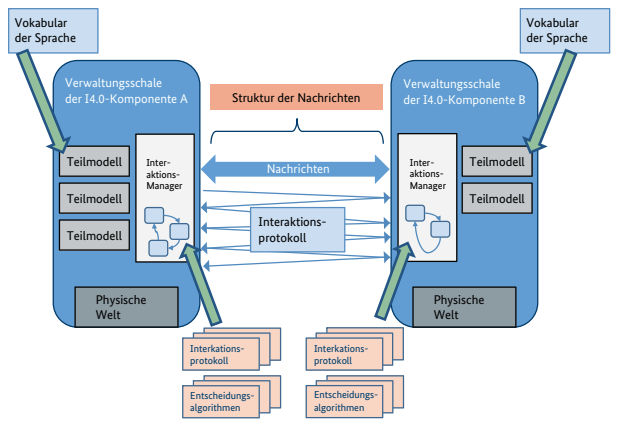
\includegraphics[scale=0.7]{content/pictures/interaction_i40_components.png}
\caption{Interaction concept of Industry 4.0 components in RAMI 4.0}
\source{\cite[p. 16]{Vialkowitsch2018VokabularI4.0-Sprache}}
\label{fig:interaction-concept-i40}
\end{figure}

\section{Classification in RAMI 4.0}

Using the outlined use cases it becomes clear, that the type of asset belonging to a \ac{I4.0} component determines its location in \ac{RAMI4.0}. In order to show the relationship between the \ac{AAS} and \ac{RAMI4.0}, the \ac{AAS} is to be classified in the six layers of \ac{RAMI4.0}. The aim of the classification is to summarize the forms of the \ac{AAS} and to highlight the associated characteristics in \ac{RAMI4.0}.

In case of the digital nameplate, the role of the \ac{AAS} in the value network is passive and therefore extends until the information layer in \ac{RAMI4.0}. Figure \ref{fig:aas-until-info-layer} graphically shows the relationship between the \ac{AAS} and \ac{RAMI4.0}. The data of the respective \ac{I4.0} component is manifested in the \ac{AAS} in the form of submodels using properties. These are stored and prepared in the information layer, enabling interoperable access by the function and business layer. Passive \ac{AAS} do not have any capabilities or functionalities and therefore have no representation in the functional or business layer. Hence, \ac{I4.0} components without a functional and business layer only contain the option for data retrieval and persistence. They can neither execute activities nor synchronize with other components in a system by means of message exchange.
\begin{figure}[h]
\centering
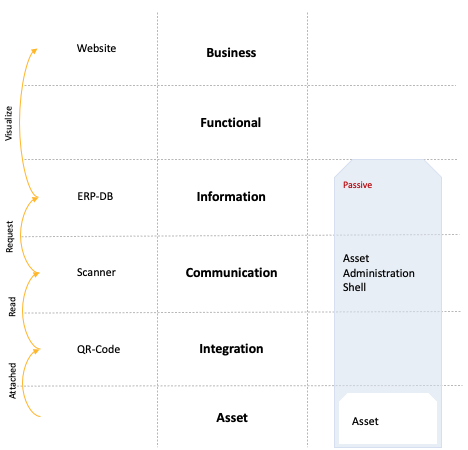
\includegraphics[width=.45\textwidth]{content/pictures/aas_rami_v1.png}
\caption{Asset Administration Shell until Information Layer}
\source{Own illustration}
\label{fig:aas-until-info-layer}
\end{figure}

The \ac{AAS} in the use case of predictive maintenance as well as plug and produce have a representation in the functional layer. The latter also includes an explicit representation in the business layer. Figure \ref{fig:aas-until-func-and-bizz-layer} graphically classifies the \ac{AAS} in \ac{RAMI4.0}, where (a) shows the use case of predictive maintenance and (b) the use case of plug and produce. Depending on whether the \ac{AAS} in the use case of predictive maintenance makes independent decisions, the \ac{AAS} are to be classified as active in regards to their role in value networks. The functionality for decision making is manifested in the business layer for active \ac{AAS}. It should be noted in both cases, that the information layer is essential for the functional layer. Without the data stored in the information layer and made available via the standardized interface of the \ac{AAS}, interoperable functionalities of the assets cannot be designed and implemented in the functional layer. The business layer provides the decision logic for executing the business and production processes based on defined business models. This includes, for example, the conditions for cost, quality and time when selecting production resources during capability checking. An important characteristic of active \ac{AAS} is, that it stores its own operating state. This is stored in a defined submodel in the information layer.

\begin{figure}[h]
\centering
\subfigure[]{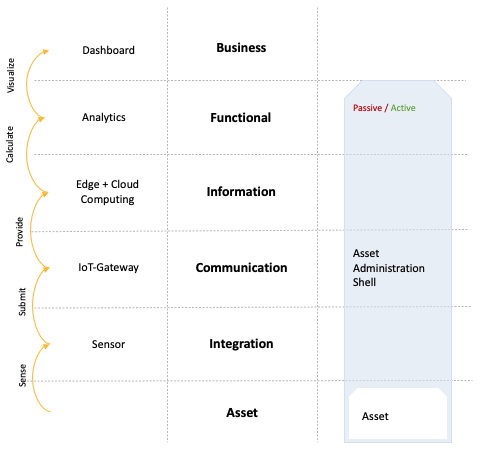
\includegraphics[width=.45\textwidth]{content/pictures/aas_rami_v2.png}}
\subfigure[]{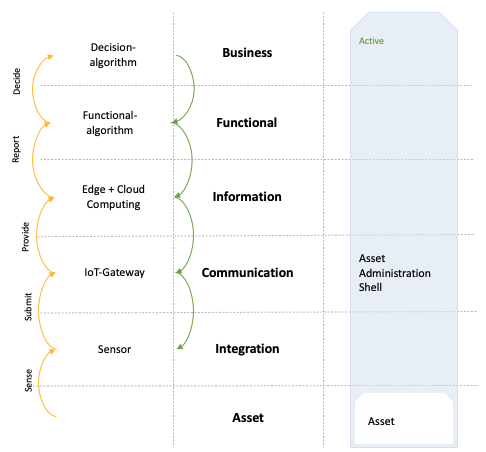
\includegraphics[width=.45\textwidth]{content/pictures/aas_rami_v3.png}}
\caption{(a) Asset Administration Shell until Functional Layer, (b) Asset Administration Shell until Business Layer}
\source{Own illustration}
\label{fig:aas-until-func-and-bizz-layer}
\end{figure}

For the type of distribution of an \ac{AAS} it can be said, that it is irrelevant whether the \ac{AAS} is provided by the asset itself, or by a central repository. However it should be noted, that for assets providing the \ac{AAS} by themselves, care must be taken to ensure \ac{I4.0} compliant communication capabilities. Otherwise, additional hardware must be attached to the asset, which can be used to realized the \ac{I4.0} compliant communication.  

For the composition of the \ac{AAS} different characteristics can be observed in the presented use cases. According to \ac{RAMI4.0}, an asset can be represented by several \ac{AAS}. This is done on the basis of the lifecycle phases \textit{type} and \textit{instance} or in order to represent different aspects of \ac{RAMI4.0} such as design, production or operation. Likewise, an \ac{AAS} can also contain or reference further \ac{AAS}. The composition does not play a significant role for the digital nameplate, as the provision of one \ac{AAS} per asset is recommended. Two different forms of composition can be observed in the use cases of predictive maintenance and plug and produce. In the case of plug and produce, each individual component in the system is described by its own \ac{AAS}. The overall system itself is being represented by an \ac{AAS} which references the individual \ac{AAS} of the components in the system \footnote{A graphical representation of this composition can bee seen in \citet[p. 246, figure 3]{Schweizer2021ProcessSystems}}. This type of composition has advantages especially for plug and produce, so that components in the system can individually be addressed and exchanged flexibly as the configuration is carried out by the component itself. In case of predictive maintenance, the type of composition cannot be derived directly from the paper of \citeauthor{Cavalieri2020AShell}. To ensure the best implementation, the following composition would be suitable: One \ac{AAS} is modeled for the entire milling station, which stores all properties and functionalities of the contained components. Although this can make the modeling of the \ac{AAS} complex in terms of submodels and bill of material, unnecessary hardware regarding networking and computation can be reduced. Similarly, network latencies can be reduced, making access to the information and functionalities in the submodels by other components more efficient. Likewise, the provision of the \ac{AAS} is simplified.
\let\cleardoublepage\clearpage
\chapter{Concept} \label{chap:concept}

In chapter \ref{chap:basics} it could be shown that the information about an asset is distributed in the six layers of \ac{RAMI4.0}. The exchange of information can take place either within one layer or between neighboring layers. The \ac{AAS}, which stores the information in submodels, is used as the central element for the exchange and orchestration of information. This is implemented with the help of the \ac{I4.0} language. In this chapter, the insights gained will be translated into a technology-independent architecture, on how to integrate \ac{BPM} in the \ac{AAS}. By doing this, general aspects will be considered first, before step-by-step instructions are given on how to implement the proposed architecture for an asset. Finally, a roadmap for companies is elaborated on how to implement \ac{I4.0} and especially the \ac{AAS} company-wide.   

\section{General aspects} \label{sec:general-aspects}
 \ac{BPM} in \ac{RAMI4.0} is distributed over the different layers. The business layer maps business models in processes, which are linked to certain conditions and prerequisites. This mapping enables the connection of loosely coupled services from the functional layer and thus the implementation of \ac{SOA}. Consequently, a control flow is created, that defines the rules for the sequence of the individual activities to be executed. The activities in \ac{BPM} correspond to the functionalities of an \ac{I4.0} component, which are defined in the functional layer and exposed via the submodels of the \ac{AAS}. Essential to the data and business objects used within a process for decision making is the information model. This is specified in \ac{RAMI4.0} by the \ac{AAS} and its submodels. The data and business objects are stored in an interoperable format in the information layer. Storing data in an interoperable format makes it possible, to exchange process participants seamlessly without adapting the process itself. As a result, side effects can be avoided. However, to be an active process participant, the \ac{AAS} must at least have a representation in the functional layer and be active in terms of their role in value networks. As a result, the information on active participants of a business process can be found in both, the functional and business layer. Based on the findings and the defined requirements, a technology-independent architecture can be derived on how \ac{BPM} can be integrated into the \ac{AAS} based on the six layers of \ac{RAMI4.0}. This is illustrated in figure \ref{fig:techn-indep-architecture}. 
 
 \begin{figure}[h]
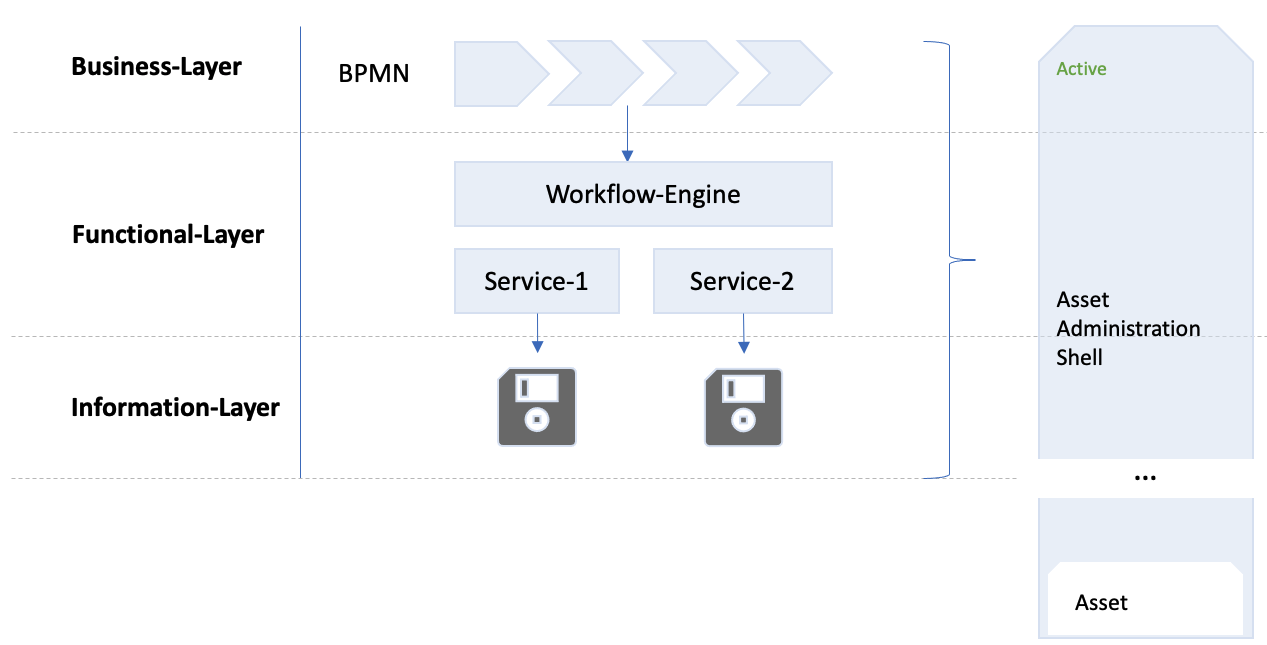
\includegraphics[scale=0.32]{content/pictures/tech_independent_architecture.png}
\caption{Technology independent architecture}
\source{Own illustration}
\label{fig:techn-indep-architecture}
\end{figure}

In the business layer, the processes representing the business models are described using \ac{BPMN}. Describing processes using \ac{BPMN} has two advantages: On the one hand, this representation creates transparency with regards to the services or activities to be executed, even for non-technical people. Likewise, non-technical people can create and manage the process mappings. On the other hand, processes can directly be executed with the help of workflow engines using \ac{BPMN}. For this purpose, the workflow engine is called with the defined process. The workflow engine then sequentially calls the activities defined in the process, by addressing the services in the functional layer. The integration of the process notation in the \ac{AAS} can be realized via submodels. Depending on the use case as well as the composition of the \ac{AAS}, the anchoring can take place in different submodels. Optimally, the anchoring of the process notation would take place in an aggregate \ac{AAS}, as described in \ref{sec:design}. In the use case of predictive maintenance, the \textit{maintenance} submodel defined by \citeauthor{Cavalieri2020AShell} could be extended by a property \textit{maintenance process}, which stores the necessary process steps to execute in the event of a technical intervention. 

The activities within a process reference the submodels defined in the \ac{AAS}. The implementation and provisioning of the submodels is realized in small independent services, that are located in the functional layer. Depending on the complexity or scope of a submodel, the service can provide both one or multiple functionalities. In the use case of \citeauthor{Cavalieri2020AShell}, two services in the functional layer would be created: A \textit{condition monitoring} and \textit{maintenance} service. These services then provide the functionalities such as \textit{set maintenance task} or \textit{get task information} via the defined interface of the \ac{AAS} \footnote{The technological implementation of the services can be done in different ways. A concrete method to instantiate services from submodels is described by \citet[p. 7]{BraunischDistributedEinleitung}. From a technical point of view, the assignment of activities to functionalities would then be done by adding URLs to the activities in \ac{BPMN}, which can then be called via HTTP by the workflow-engine.}. However, when implementing workflow engines, care must be taken not to create a too strong coupling between the functional layer services and the workflow engine. By doing so, it would be worth considering whether the workflow engine should be replaced by a message-oriented infrastructure using a message broker. The discussion whether to use a message-oriented infrastructure or workflow engines is out of scope of this thesis. The intention is to present a design pattern and not a complete architecture.

\section{Design} \label{sec:design}

The described architecture in \ref{sec:general-aspects} is of rather abstract nature, which does not directly indicate the necessary steps for implementation. In the following section, step-by-step instructions will be given on how to implement this. The architecture will be explained on the basis of the use case of predictive maintenance from \citeauthor{Cavalieri2020AShell}. While the paper from \citeauthor{Cavalieri2020AShell} only deals with creating the information model based on the \ac{AAS}, this approach extends their findings by describing a \ac{RAMI4.0} compliant architecture for the implementation of predictive maintenance which conforms to the one elaborated in \ref{sec:general-aspects}. The first step in the implementation is the definition of the composition. The composition determines how the individual assets are digitized. This step is of particular importance as it directly influences steps two and three. In a second step, it must be defined, how the connection between the physical and virtual environment can be established with the help of information technologies. To this end, a corresponding technology must be defined for each layer in \ac{RAMI4.0}. Afterwards, an information model must be derived for each asset in the system,  that describes the properties and functionalities of the asset. The information model is then manifested and transferred into the submodels of the \ac{AAS}. In a final step, the processes specified by the business model are modeled using \ac{BPM} and the individual activities of the process are linked to the respective submodel in the \ac{AAS}.

\textbf{Step 1: Composition definition}

When defining the composition, the use case to be realized and the assets to be digitized must first be considered. In case of an asset group, the individual components must be identified and considerations must be given to whether they require their own \ac{AAS} or not. In order to derive a decision, it must be evaluated whether the component should be active or passive in terms of their role in value networks and to what extent the functionalities of the asset should be represented independently in the overall system. As already outlined in \ref{sec:assetadministrationshell}, an asset in \ac{RAMI4.0} can be described by several \ac{AAS}. Likewise, an \ac{AAS} can contain further \ac{AAS}. This results in a multitude of combinations for digitizing assets. For example, the milling station in the present case can be implemented as one large \ac{AAS}, in which all sub-components, such as the robot's gripper arm, are included. It is also conceivable that one \ac{AAS} is created for each individual sub-component, which are then aggregated in the \ac{AAS} of the overall system. The difficulty in digitizing assets in \ac{RAMI4.0} using the \ac{AAS} is hence to find the right abstraction based on the scenario the asset is used. 

In the following, three possible forms of composing the milling station will be presented, based on which the advantages of each form will be discussed. Finally, a conclusion is drawn which composition is most suitable for predictive maintenance. Figure \ref{fig:aas-modeling-alternatives} graphically shows the three forms.

\begin{figure}[h]
\centering
\subfigure[]{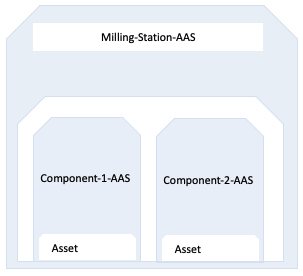
\includegraphics[width=.3\textwidth]{content/pictures/aas_version_1.png}}
\subfigure[]{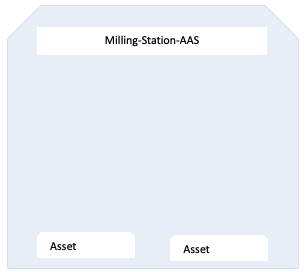
\includegraphics[width=.3\textwidth]{content/pictures/aas_version_2.png}}
\subfigure[]{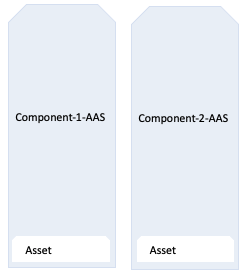
\includegraphics[width=.3\textwidth]{content/pictures/aas_version_3.png}}
\caption{Modelling alternatives for digitizing assets: (a) Asset Administration Shell from the individual components is aggregated on the root level, (b) all components are covered by a single Asset Administration Shell, (c) each component exposes its own Asset Administration Shell}
\source{Own illustration}
\label{fig:aas-modeling-alternatives}
\end{figure}

Figure \ref{fig:aas-modeling-alternatives} (a) shows that each component in the milling station is modeled with its own \ac{AAS}. The individual components are aggregated into one \ac{AAS} which is then exposed to the network. This type of composition has advantages in reducing complexity while modelling the individual submodels of the \ac{AAS}. This is especially the case if the components of the milling station are delivered by different manufacturers. To this end, each component manufacturer equips its component with an \ac{AAS}. The operator of the asset would then aggregate the individual \ac{AAS} into the milling station \ac{AAS}, which exposes the required properties and functionalities through one interface. In addition to the reduced complexity in modelling, this type of composition has advantages in \ac{SOA}. By addressing one component in the network, communication overhead and complexity can be reduced.

In Figure \ref{fig:aas-modeling-alternatives} (b) all properties and functionalities of an asset are modeled in one \ac{AAS}. For assets with many sub-components, this type of composition can quickly lead to high complexity in the submodels. However, this type of composition has the advantage, that hardware requirements can be reduced. This is especially the case for \ac{AAS}, that are active but do not have \ac{I4.0} communication capabilities. All functionalities and properties could be provided via one \ac{SBC} or \ac{OPCUA} server.

Figure \ref{fig:aas-modeling-alternatives} (c) shows the type of composition, which has the least coupling between the individual components. It is similar to the composition in \ref{fig:aas-modeling-alternatives} (a), without the aggregation in the milling station \ac{AAS}. For this purpose, each component of the milling station provides its functionalities and properties in the network itself. This type of composition has particular advantages when optimizations are to be realized with regard to latency or information access. For example, it is conceivable that the \ac{AAS} of component 1 is provided by the component itself using \ac{OPCUA} at the edge. The provisioning of component 2's \ac{AAS} can be realized in the cloud, since latencies in communication play a minor role. 

Variant (a) is particularly recommended for the implementation of predictive maintenance, as it offers the greatest flexibility in terms of provisioning and implementation of functionalities in cloud and edge and at the same time offers the possibility of aggregation reducing network overhead. The two options, cloud and edge, of provisioning an \ac{AAS} are especially important for use cases that work with real-time data.

\textbf{Step 2: IT-Platform}

After the type of digitization has been determined in step one, the connection between the physical and virtual world  must be established in a second step. For this purpose, the technical resources that meet the requirements for communication and processing of data must be selected. The requirements are derived directly from the selected composition. Figure \ref{fig:technology-map} provides an overview of possible technologies that are available for realizing different compositions. The outlined technologies are aligned with the layers of \ac{RAMI4.0}.

\begin{figure}[h]
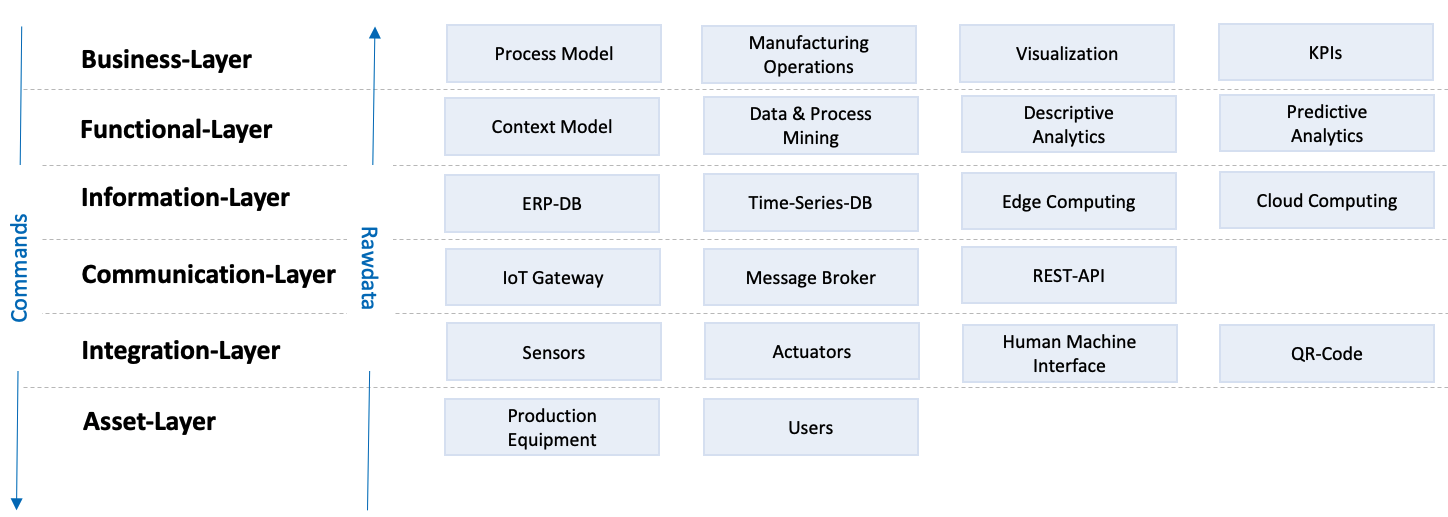
\includegraphics[scale=0.31]{content/pictures/rami_40_tech_mapping.png}
\caption{Technology map in the layers of RAMI4.0}
\source{Own illustration}
\label{fig:technology-map}
\end{figure}

In most cases, the asset is integrated into the virtual world using sensors or actuators in the integration layer. The generated data is then forwarded via an \ac{IIOT} gateway in the communication layer with \ac{I4.0} communication capabilities to the information layer, which stores and further processes the data in the \ac{AAS}. For the processing of time series and real-time data in the information layer, time series databases are the best choice, whereas relational databases are suitable for the storage of structural data. In the use case of predictive maintenance, a decision in favor of composition (a) from step one was made. Consequently, a separate \ac{AAS} is created for each component in the system, which is then combined in the system \ac{AAS}. This type of composition allows each component to use the optimal selection of technology to realize its functionality. This means that, for example, component 1 provides its data via an \ac{IIOT} gateway, while component 2 does so via a message broker using \ac{MQTT}. 

In order to derive a suitable selection of technologies, the requirements of the individual components must be defined in terms of networking, latency and required computing power. While a concrete decision regarding the requirements always depends on the specific environment, predictive maintenance is to be implemented, figure \ref{fig:technology-map-pred-maint} shows a selection of technologies that could be considered for implementing predictive maintenance. 

\begin{figure}[h]
\centering
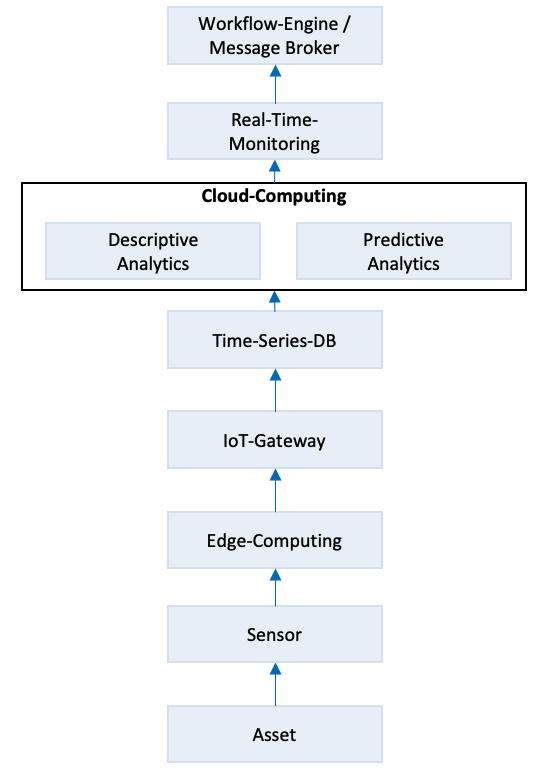
\includegraphics[width=.5\textwidth]{content/pictures/tech_map_pred_maintenance.png}
\caption{Technology map predictive maintenance}
\source{Own illustration}
\label{fig:technology-map-pred-maint}
\end{figure}

The two elements Cloud-Computing and Edge-Computing are particularly noteworthy. The provisioning of functionalities of the \ac{AAS} that require low latency can be realized at the edge. Functionalities that require intensive computing power but have lower latency requirements can be implemented in the cloud. The interoperable description of the functionalities in the submodels of the \ac{AAS} likewise allows the technologies to be exchanged seamlessly. Functionalities that are realized in the cloud can also be executed on the edge, given that the requirements regarding computing capacities are met.

\textbf{Step 3: Design of \ac{AAS}}

After defining the composition in step one and the technological infrastructure in step two, step three involves designing the information model for the individual elements of the composition. In doing so, the individual properties and functionalities of the asset must be transferred into submodels according to the property principle. For this purpose, it is suitable to divide the properties and functionalities of the asset into logical blocks. A logical block is a grouping that represents a specific aspect of the asset. If possible, standardized templates should be used to model interoperable properties and functions. For all properties that are not already provided in templates, standardized properties such as eclass should be used. \citet[p. 8, 10]{Cavalieri2020AShell} already provide a comprehensive information model, so that the modeling will not be shown in detail in this thesis.  However, a good possibility to get started with the design of an information model is provided by the package explorer through the Industry 4.0 platform \footnote{The package explorer is currently only available for the Windows platform and can be downloaded here: https://github.com/admin-shell-io/aasx-package-explorer}.

\textbf{Step 4: Design of business processes}

In the final step, the business model must be transformed into a process model with the help of \ac{BPMN}. To do this, the data needed to make decision within the process must be defined, as well as the activities that are to be performed. The activities of the process are linked to the services from the functional layer, in which the functionalities of the asset are mapped. It is recommended to define a process segment for each identified logical block from step three. Figure \ref{fig:pred-maintenance} shows an example process for predictive maintenance, which can be used to orchestrate the individual services in the functional layer.

\begin{figure}[h]
\centering
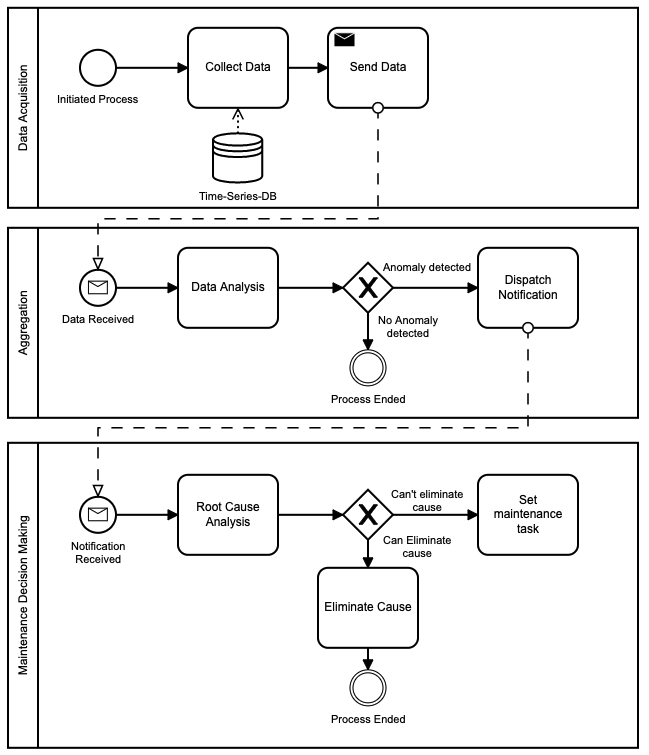
\includegraphics[width=.6\textwidth]{content/pictures/business_process_notation.png}
\caption{Business process for predictive maintenance}
\source{Own illustration}
\label{fig:pred-maintenance}
\end{figure}


\section{Roadmap to Industrial Digital Twin}
The instructions for implementing the \ac{AAS} and associated business processes shown in section \ref{sec:design} are applicable to an asset or asset group. In order to not limit the implementation to one asset or asset group, a roadmap is necessary that holistically enables the transformation of companies towards \ac{I4.0}. The introduction of \ac{RAMI4.0}, the \ac{AAS} and the accompanying transformation towards \ac{SOA} can present companies with a challenge. Companies will not be able to adopt directly the development of active \ac{AAS} and adapt their business processes accordingly as described in the previous chapter. Rather, a step-by-step transformation will be required to adapt an organization to the \ac{SOA} proposed by \ac{RAMI4.0} as well as the \ac{AAS}. To this end, the first step is to validate the already implemented measures and derive a development plan. A good framework for classifying and evaluating the current adoption of \ac{RAMI4.0} is provided by the maturity index, developed by \cite[p. 15]{Schuh2020IndustrieAcatech}. The maturity index consists of six successive steps through which adoption of \ac{I4.0} can be evaluated. These are \textit{Compute}, \textit{Connect}, \textit{Visible}, \textit{Transparent}, \textit{Predict} and \textit{Adapt}. \textit{Compute} describes the use of separate, unrelated information technologies, such as \ac{CNC}, to increase efficiency and reduce error rates \cite[p. 15]{Schuh2020IndustrieAcatech}. While \textit{Compute} introduces isolated information technologies, \textit{Connect} is concerned with the connection of individual production resources on the shop floor via \ac{API}s, which attempt to map the business processes. This can be done with the help of tools like \ac{MES} or \ac{ERP} \cite[p. 16]{Schuh2020IndustrieAcatech}. The two successive steps are referred to by the authors as the digitization, which lay the foundation for the implementation of \ac{I4.0} and the \ac{AAS}. The first step towards implementing \ac{I4.0} is \textit{Visible}. In this step, real-time capabilities are implemented for the assets on the shop floor. The real-time capabilities enable human decision making on based on the current status of the asset. \textit{Visible} also enables the connection of different data systems in the company such as \ac{MES} with \ac{ERP} \cite[p. 17]{Schuh2020IndustrieAcatech}. The available real-time-data is afterwards aggregated, analyzed and related data sets are linked to it. Therefore, this step is called \textit{Transparent}. The aim of this step is to use Big Data technologies to identify errors, monitor assets and establish impact correlations between the individual data sets. \textit{Predict} is defined as the ability to make predictions about future behaviour from historical and real-time data, so that potential problems can be identified in advance and appropriate action can be taken \cite[p. 19]{Schuh2020IndustrieAcatech}. If the actions to be taken are decided and executed by a system component itself without human interaction, one speaks of \textit{Adapt}, which represents the final step in the development of \ac{I4.0}. 

While the index represents a maturity model, \ac{RAMI4.0} provides a reference model with which companies can achieve the vision of \ac{I4.0}. However, \ac{RAMI4.0} only provides the organizational and technical parameters, but not a medium for evaluating the technical and organizational transformation. To assess the transformation of a company and thus the maturity level, the individual steps of the index are plotted on the Y-axis and the layers of \ac{RAMI4.0} on the X-axis. This makes it possible to derive a roadmap for the implementation of the individual layers of \ac{RAMI4.0} and to evaluate the opportunities it brings. Figure \ref{fig:roadmap} graphically establishes the relationship between the maturity model and \ac{RAMI4.0}.

\begin{figure}[h]
\centering
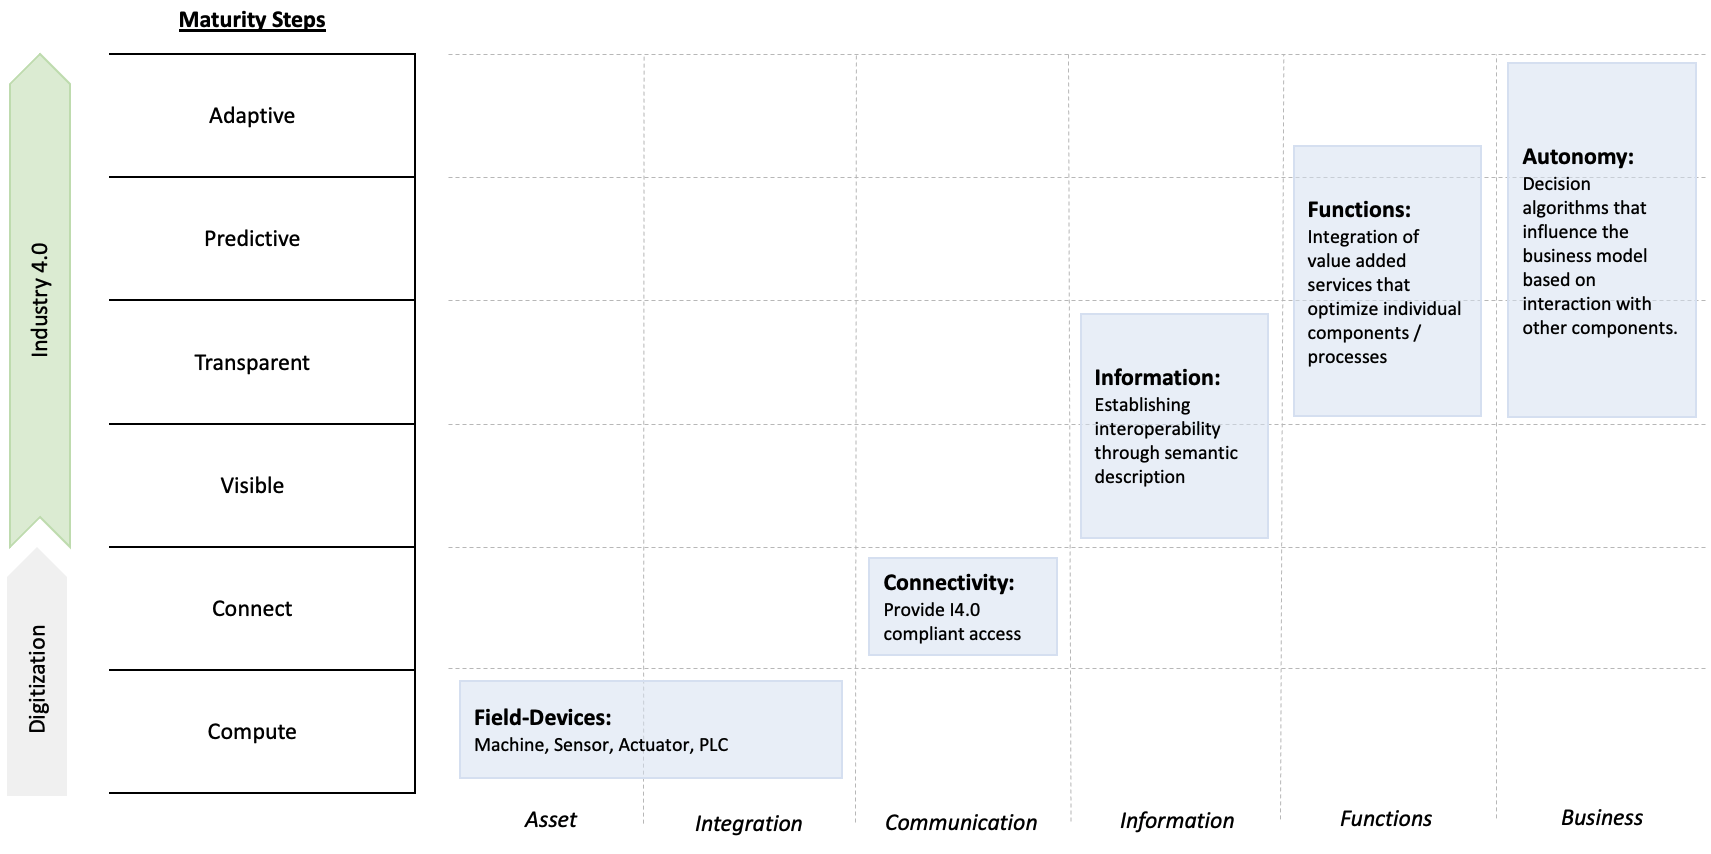
\includegraphics[scale=0.25]{content/pictures/rami_roadmap.png}
\caption{Roadmap for implementing RAMI4.0 based on the maturity index}
\source{Own illustration}
\label{fig:roadmap}
\end{figure}

The first two steps to enable the digitization of assets are computerization and connectivity. For this purpose, the assets must be equipped with sensors, actuators or PLCs in the asset layer of \ac{RAMI4.0}. In a second step, these must be connected with each other through \ac{I4.0} compatible technologies, such as \ac{IIOT} gateways. This includes, for example, retrofitting assets that do not currently have \ac{I4.0} communication capabilities, or replacing them with \ac{I4.0} compatible assets. Once the foundation for \ac{I4.0} has been laid through digitization, the assets can be described with the help of the \ac{AAS} in order to establish interoperability. The introduction of the \ac{AAS} will enable companies for the first time to view and store data from the shop floor in real-time. Given that the data is prepared graphically, for example in a dashboard, initial conclusion or measures can be derived based on the collected and stored data. While this data is primarily suitable for optimizing internal processes and reducing costs, the first added value for customers can be achieved by introducing predictive capacities in the functional layer. For this purpose, the previously purely passive \ac{AAS} must be converted into active \ac{AAS} and the functionalities must be mapped in the submodels. The functionalities of the submodels must then be provided in the form of services on the functional layer. By introducing \ac{BPM} and mapping business models in processes in the business layer, \textit{Adapt} can be realized. For this purpose, the processes are executed with the help of workflow engines, which call the services in the functional layer. This type of interaction then leas to decisions being made autonomously, with the aim of achieving end-to-end optimization of all processes in the company. 

An important insight that emerges from the roadmap is that the implementation of \ac{RAMI4.0} and the \ac{AAS} does not have to happen all at once. Rather, this can be done step by step. However, when implementing the individual steps, one should always be clear about the added value that can be realized as a result.
\let\cleardoublepage\clearpage
\chapter{Summary} \label{chap:summary}

\section{Conclusion}
This thesis deals with the \ac{DT} in the context of \ac{I4.0}. Specifically, it examines the role of the \ac{DT} in value networks and how business and production processes can be mapped in it, so that it becomes the central control element in \ac{CPS}. To this end, a first chapter provides an introduction to value networks and their realization in the context of \ac{I4.0}. It shows, that the realization of value networks in \ac{I4.0} is predominantly technology-based and takes place on platforms. The realization of value networks via platforms in \ac{I4.0} opens up new opportunities for companies. However, the possibilities that can be realized via \ac{I4.0} platforms often go hand in hand with complex relationships between the partners. This is on the one hand because the technology-based approach introduces new processes and interfaces that are needed to exchange data between the partners. On the other hand, there are new participants in value creation, especially from the digital ecosystem, offering specialized services. To make the complexities manageable, a reference architecture model, namely \ac{RAMI4.0}, is presented. \ac{RAMI4.0} makes it possible to map the complex relationships between the partners of a value network and enables the interdisciplinary technical data description of an asset over the entire life cycle. With this in mind, \ac{RAMI4.0} introduces three dimensions to simplify the description of assets. These are layers, life cycle and value streams as well as hierarchy levels. The information about an asset is stored in the layers, the asset's life cycle is mapped in the life cycle and value stream, and the connection between the asset and the connected world is established in the hierarchy levels. A central element for the data-based technical description of assets in \ac{RAMI4.0} is the \ac{I4.0} component with its \ac{AAS}. In the context of \ac{I4.0}, the \ac{AAS} corresponds to the digital twin and allows a technology-independent description of assets. For this purpose, a general introduction to \ac{DT} in the context of \ac{CPS} is given and the connection to the \ac{I4.0} component and \ac{AAS} is established.  In a second chapter, a closer look at the \ac{AAS} and its characteristics is taken. The \ac{AAS} is a technology-independent description of assets with the help of standardized submodels. The characteristic features of an \ac{AAS} are illustrated on the basis of three use cases: the digital nameplate, predictive maintenance as well as plug and produce. Next to the description of the properties in submodels, three important features of the \ac{AAS} are identified: These are the role of the \ac{AAS} in value networks, the distribution and their composition. The communication between the individual components in an \ac{I4.0} system is realized with the help of the \ac{I4.0} language, which is manifested in the submodels of the \ac{AAS}. The communication between the individual \ac{AAS} thus enables components in a system to act autonomously by responding to requests from other components and making decision based on this. This makes the \ac{AAS} the central control element in \ac{I4.0} systems. In the last chapter of the thesis, the gained knowledge is transferred into a technology independent architecture concept. For the implementation of the concept, a step-by-step guide is introduced, which establishes the connection between the \ac{AAS} and \ac{BPM}. Finally, a roadmap is introduced that can be used to derive the development path of companies towards \ac{RAMI4.0} and the introduction of the \ac{AAS}.

In the course of the thesis, the questions raised in \ref{sec:research-question} can be answered as follows:

\begin{itemize}
    \item [] \textbf{Question 1:} \textit{How can \ac{BPM} be classified in the six layers of \ac{RAMI4.0}?}
    
    To answer the question, the layers in \ac{RAMI4.0} are examined in more detail with regard to their information stored and the flow of information between the individual layers. It is shown that the information in the layers of \ac{RAMI4.0} can be exchange either within the layer itself or between neighboring layers. The information layer is particularly worthy to mention. The information layer is a central layer in the reference model, since it stores and processes the data transmitted from the communication layer in an interoperable manner. This lays the foundation for the implementation of services in the functional layer and the mapping of business models in the business layer. Contrary to the definition of \ac{RAMI4.0}, it can thus be stated that \ac{BPM} includes three layers: the information, the functional and the business layer. These are mutually dependent. To implement business and production processes according to \ac{RAMI4.0}, the information, functional and business layers must be provided. 
    
    \item [] \textbf{Question 2:} \textit{How can a link between a process and the required services involved in it be established with the help of the \ac{AAS}?}
    
    In order to answer the question, the structure, contents and characteristic features of the \ac{AAS} are elaborated. Likewise, a look is taken at the interaction of \ac{I4.0} components that describe a business model through a process. It is shown that the mapping of functionalities and properties of a physical asset is realized with the help of standardized submodels in the \ac{AAS}. A submodel represents exactly one general or specific aspect of an asset. In order to establish the relationship between a process and the services involved with the help of the \ac{AAS}, the \ac{AAS} must take at least and active role in value networks. This means that the \ac{AAS} has a representation in the functional layer of \ac{RAMI4.0} and provides its functionalities in the form of services. Its active role within value networks allows the \ac{AAS} to communicate and make decisions based on the interaction with other components in the network. Passive \ac{AAS} cannot be active participants in a process because they have no representation in the functional layer.
    
    \item[] \textbf{Question 3:} \textit{How can a concrete integration of \ac{BPM} in the \ac{AAS} be realized based on the six layers of \ac{RAMI4.0}?}
    
    The integration of \ac{BPM} into the \ac{AAS} based on the six layers of \ac{RAMI4.0} can be realized via submodels of the \ac{AAS} by anchoring a process description in the \ac{AAS} using \ac{BPMN}. By doing so, the business models defined in the business layer are translated into processes that are modeled in \ac{BPMN}. The execution of the processes can be performed using workflow engines. To this end, the workflow engine calls the activities defined in the process sequentially. An activity corresponds to exactly one functionality that is defined in a submodel of the \ac{AAS} and exposed via the functional layer of \ac{RAMI4.0}. The actual implementation of the integration takes place in four successive steps: Definition of composition, design of IT-platform, design of information model and modeling of the business and manufacturing process. The composition determines the digitization of the asset: One \ac{AAS} for each component, or one \ac{AAS} that composes multiple components. The IT-platform defines the technology for the implementation of the individual layers, and the design of the information model defines the properties and functionalities of the asset, which is transferred into submodels of the \ac{AAS}.

\end{itemize}

\section{Critical Reflection}

The thesis tries to build a bridge between the technical and business aspects in \ac{RAMI4.0} and its containing \ac{AAS}. During the elaboration, it was found that \ac{RAMI4.0} is a complex reference model that tries to company many technical and business aspects, which makes it difficult to derive a generally valid and understandable architecture that takes all the relevant requirements defined into account. It is a great challenge to prepare and present the essential information of the individual aspects in a holistic way from a business and technical perspective. As a result, the acceptance and implementation of \ac{RAMI4.0} are low so far. To increase acceptance and simplify the implementation of \ac{RAMI4.0} and the \ac{AAS}, a further breakdown of the relevant aspects must be made. To do so, the technical and business aspects of the individual layers of \ac{RAMI4.0} must be made available in more detail and in a simplified form. This thesis can be used as a starting point, as it provides an overview and first approaches to implementation. This requires further specification of the individual steps defined in chapter \ref{sec:design} for implementing the proposed architecture. To do so, the technological and business aspects must be addressed separately. For the technical aspect,  in particular, the information, functional and business layers of \ac{RAMI4.0} are to be considered more closely and the role of the \ac{AAS} hereby. To to this, the technical requirements for the individual layers must be specified in more detail and the defined approaches must be tested independently and their feasibility evaluated in prototypes. For the economic analysis, the business value in particular must be worked out and calculated, which can be realized during the implementation of \ac{RAMI4.0} and the \ac{AAS}. In conclusion, it can be said, that the question of this thesis represents a very extensive subject area, so that the result of the thesis provides more of an overview with initial approaches, rather than a concretely applicable concept. In order to develop a concrete application concept, the question would have had to be limited to a specific field of application.
\let\cleardoublepage\clearpage


% Literaturverzeichnis
\singlespacing
\bibliographystyle{abbrvnat}
\bibliography{bibtex}

% Eidesstattliche Erklärung
\chapter*{Eidesstattliche Erklärung\markboth{Eidesstattliche Erklärung}{}}
% Eintrag in das Inhaltsverzeichnis 
\addcontentsline{toc}{chapter}{Eidesstattliche Erklärung}

Ich versichere, dass ich die vorstehende Arbeit selbstständig verfasst und hierzu
keine anderen als die angegebenen Hilfsmittel verwendet habe. Alle Stellen der Arbeit die 
wörtlich oder sinngemäß aus fremden Quellen entnommen wurden, sind als solche kenntlich gemacht.
\\
\\
Die Arbeit wurde bisher in gleicher oder ähnlicher Form in keinem anderen
Studiengang als Prüfungsleistung vorgelegt oder an anderer Stelle
veröffentlicht.
\\
\\
Ich bin mir bewusst, dass eine falsche Erklärung rechtliche Folgen haben kann.

\vspace*{1.5cm} \par
\line(1,0){200} \par
\docOrt, \docAbgabedatum ~~\docVorname~\docNachname


%Zurücksetzen \chaptermark
\let\chaptermark\oldchaptermark


\end{document}      